\setchapterpreamble[u]{\margintoc} 
\chapter{Modéliser un mécanisme} 
\section{Analyser un mécanisme en utilisant un graphe de liaisons} 
\section{Simplifier un mécanisme en utilisant une liaison équivalente} 
\section{Évaluer l'hyperstatisme d'un mécanisme} 
\graphicspath{{\repStyle/png/}{../CHS/CHS-03-HS/64_EPAS/images/}} 
\normaltrue \difficilefalse \tdifficilefalse
\correctiontrue
%\UPSTIidClasse{11} % 11 sup, 12 spé
%\newcommand{\UPSTIidClasse}{11}

\exer{Système EPAS $\star$ \label{CHS:03:B2:16:64}}
%% CCP MP 2007
\setcounter{question}{0}\marginnote{\xpComp{CHS}{03}}%\UPSTIcompetence[2]{B2-16}
\index{Compétence CHS-03}\index{Compétence B2-16}

\index{EPAS}
\index{Hyperstatisme}

\ifcorrection
\else
\marginnote{\textbf{Pas de corrigé pour cet exercice.}}
\fi

\ifprof
\else
On s'intéresse à l'échelle pivotante équipant un camion de pompier. On donne un schéma cinématique du système de manoeuvre du parc échelle.
 
\begin{figure}[h!]
\centering
    \begin{subfigure}[c]{0.45\textwidth}
        \centering
        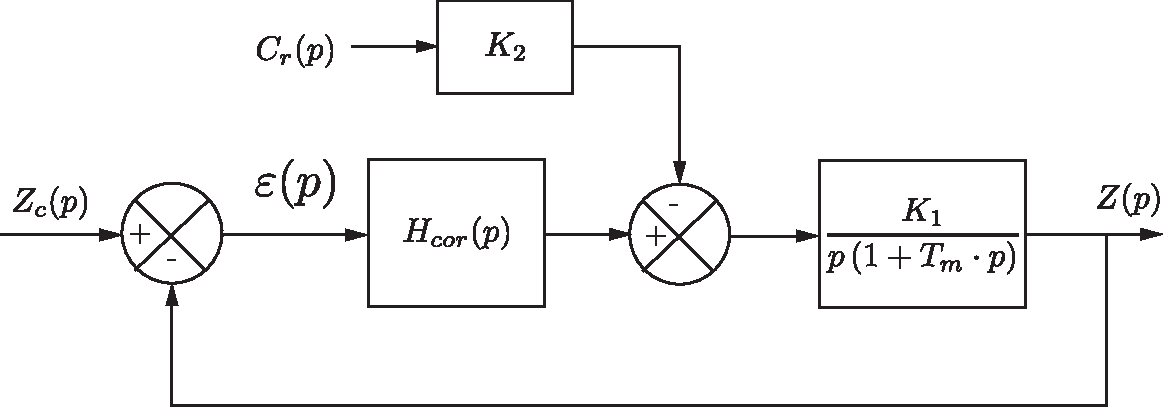
\includegraphics[width=\linewidth]{64_01.png}
    \end{subfigure}%
    \hfill
    \begin{subfigure}[c]{0.45\textwidth}
        \centering
        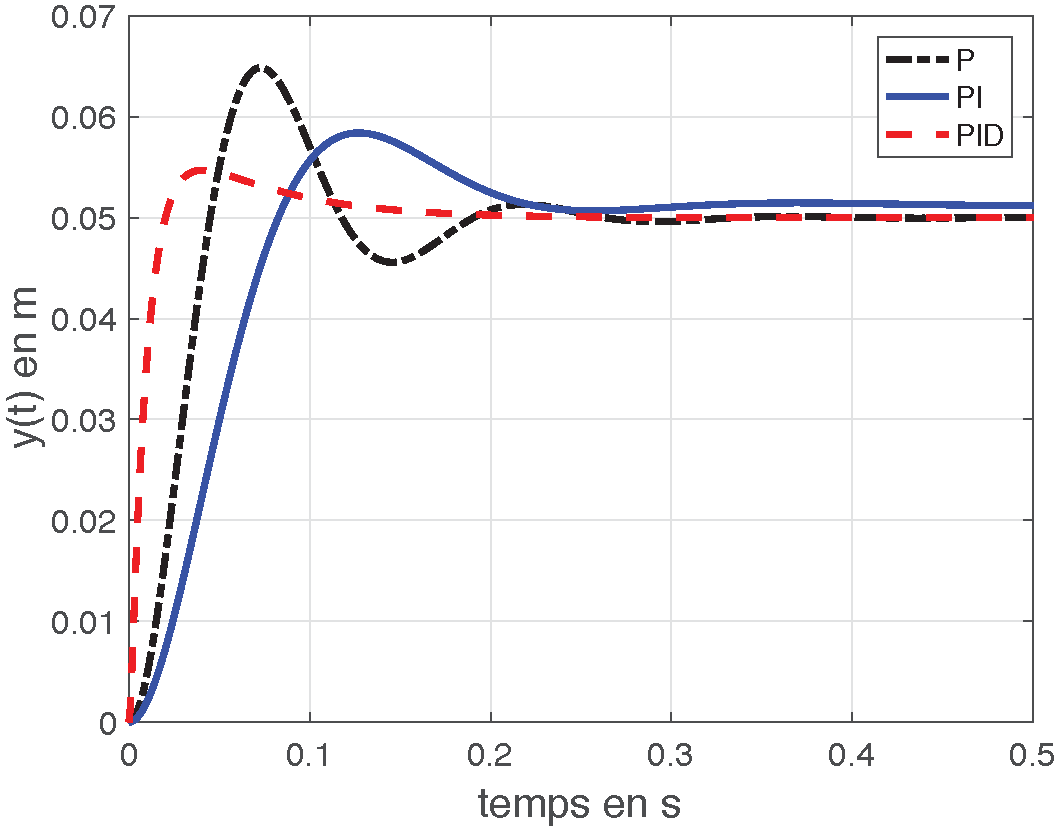
\includegraphics[width=\linewidth]{64_02.png}
    \end{subfigure}
    %\caption{Caption place holder}
\end{figure}
\fi

\question{Réaliser le graphe des liaisons.}
\ifprof

\begin{center}
\includegraphics[width=10cm]{64_01_cor}
\end{center}

\else 
\fi

\question{Déterminer le degré d’hyperstatisme de ce mécanisme.}
\ifprof
Détermination des mobilités : 
\begin{itemize}
\item rotation de l'ensemble des pièces en rotation autour de $\vect{y}$ grâce à la pivot entre 0 et 1;
\item rotation de la pivot entre 1 et 2 par mouvements opposés des pivots glissant 4--5 et 4'--5';
\item rotation de la pivot entre 2 et 3 par mouvements simultanés des pivots glissant 6--7 et 6'--7'.
\end{itemize}
On a donc $m=3$. 

\textbf{Méthode cinématique : }
\begin{itemize}
\item nombre de cycles : 15 liaisons et 12 solides, $\gamma = L- S + 1 =4$;
\item nombre d'équations cinématiques: $E_c = 6\times 4 = 24$;
\item nombre d'inconnues cinématiques : $I_c = 4 \times 2+ 11 \times 1 = 19$;
\item hyperstaticité : $h=m-I_c + E_c = 3 -19 + 24 = 8$.
\end{itemize}


\textbf{Méthode statique : }
\begin{itemize}
\item nombre d'équations statiques : $E_s = 6\times 11 = 66$;
\item nombre d'inconnues statiques : $I_s = 4 \times 4+ 11 \times 5 = 71$;
\item hyperstaticité : $h=m-E_s + I_s = 3 -66 + 71 = 8$.
\end{itemize}


\else 
\fi

\question{Proposer des modifications qui permettraient de le rendre isostatique.}
\ifprof
On va chercher à rendre le système isostatique tout en conservant une même architecture pour des branches en parallèles.

Dans le cycle 1--2--5--4--1 pris indépendamment du reste du mécanisme on a :
\begin{itemize}
\item $m=1$;
\item $I_c = 1+1+2+1 = 4$;
\item $E_c =6 \times 1$;
\item $h_1 = m-I_c +E_c = 2 -4 +6 =4$. 
\end{itemize}

En remplaçant la pivot entre 1 et 4 par une linéaire annulaire, on ajoute 3 inconnues cinématiques et 1 mobilité. 
On a donc $h_1 = 2$. On peut faire le même changement pour les liaisons 4' -- 5', 2 -- 6, 2 -- 6'.

On a donc :
\begin{itemize}
\item $m=7$
\item nombre de cycles : 15 liaisons et 12 solides, $\gamma = L- S + 1 =4$;
\item nombre d'équations cinématiques: $E_c = 6\times 4 = 24$;
\item nombre d'inconnues cinématiques : $I_c = 4 \times 2+ 7 \times 1+ 4 \times 4 = 31$;
\item hyperstaticité : $h=m-I_c + E_c = 7 -31 + 24 = 0$.
\end{itemize}
  
(Vérifier que les linéaires annulaires n'ajoutent pas des mobiltés supplémentaires...)

\else 
\fi
 
 

\ifprof
\else
\ifcolle
\else
\marginnote[-4cm]{
\begin{solution}
 \begin{enumerate}
\item .
\item $h=8$.
\item .
 \end{enumerate}
\end{solution}} 
\fi

\marginnote{\footnotesize{Corrigé  voir \ref{CHS:03:B2:16:64}.}}
\fi 
 
\graphicspath{{\repStyle/png/}{../CHS/CHS-03-HS/69_TrainA350/images/}} 
\normaltrue \difficilefalse \tdifficilefalse
\correctiontrue
%\UPSTIidClasse{11} % 11 sup, 12 spé
%\newcommand{\UPSTIidClasse}{11}

\exer{ Train avant d'A350 -- 900$\star$ \label{CHS:03:B2:16:69}}
%% CCP MP 2007
\setcounter{question}{0}\marginnote{\xpComp{CHS}{03}}%\UPSTIcompetence[2]{B2-16}
\index{Compétence CHS-03}\index{Compétence B2-16}

\index{Train d'atterrissage A350}
\index{Hyperstatisme}

\ifcorrection
\else
\marginnote{\textbf{Pas de corrigé pour cet exercice.}}
\fi

\ifprof
\else
La configuration du train d’atterrissage de l’avion A350-900 est de type tricycle avec :
\begin{itemize}
\item deux atterrisseurs principaux (gauche et droit) attachés sur la voilure, légèrement à
l’arrière du centre de gravité $G$ de l’avion et de part et d’autre du plan de symétrie
vertical $\left(O, \vect{x}, \vect{z}\right)$ de l'avion. Ils supportent l’essentiel du poids de l’avion ;
\item un atterrisseur auxiliaire situé sous le nez de l’avion, qui assure l’équilibre longitudinal
de l’avion au sol et permet de manoeuvrer.
\end{itemize}
Les atterrisseurs principaux sont équipés de quatre roues chacun, tandis que
l’atterrisseur auxiliaire est équipé de deux roues.



\begin{marginfigure}
\includegraphics[width=\linewidth]{69_01}
\end{marginfigure}

Les mobilités entre les différents éléments de l’avion (roues,
fuselage…) ne sont pas considérées ; ces éléments ne forment donc qu’une seule
classe d’équivalence désignée « avion ».

\fi

On modélise chacune des 8 liaisons au sol par une liaison ponctuelle (sphère-plan).
\question{Réaliser le graphe des liaisons.}
\ifprof
\begin{center}
\includegraphics[width=5cm]{69_01_cor}
\end{center}
\else 
\fi

\question{Déterminer le degré d’hyperstatisme d’une modélisation de la liaison avion-sol
dans laquelle chaque contact roue-sol serait considéré ponctuel.}
\ifprof
La liaison de l'avion avec le sol est assimilabe à une liaison appui-plan de normale $\vect{z}$. Il y a donc 3 mobilités (1 rotation autour de $\vect{z}$, 1 translation selon $\vect{x}$ et 1 translation suivant $\vect{y}$.

En utilisant une méthode statique, on a $h=m-E_s+I_s$ avec : 
\begin{itemize}
\item  $m=3$;
\item $E_s = 1\times 6 = 6$ (on ne peut isoler que l'avion);
\item $I_s = 10 \times 1 = 10$ (8 liaisons ponctuelles avec 1 inconnue statique par liaison).
\end{itemize}
En conséquences, $h = 3-6+10 =7$. 

En utilisant une méthode cinématique, on a $h=m-I_c+E_c$ avec : 
\begin{itemize}
\item  $m=3$;
\item $E_c = \gamma \times 6 = (10-2+1) \times 6 = 54$ (on ne peut isoler que l'avion);
\item $I_c = 10 \times 5 = 50$ (8 liaisons ponctuelles avec 5 inconnues cinématiques par liaison).
\end{itemize}
En conséquences, $h = 3-50+54 =7$. 

\else 
\fi

Pour simplifier l’étude, les actions mécaniques de contact entre chaque atterrisseur et
le sol sont modélisées globalement par un effort ponctuel vertical. Ainsi la modélisation
introduit trois liaisons ponctuelles de normales $(A, \vect{z})$ (atterrisseur
auxiliaire), $(P_g, \vect{z})$ (atterrisseur principal gauche) et $(P_d, \vect{z})$ (atterrisseur principal droit).

\question{Démontrer que ce modèle simplifié est isostatique.}
\ifprof

En utilisant une méthode statique, on a $h=m-E_s+I_s$ avec : 
\begin{itemize}
\item  $m=3$;
\item $E_s = 1\times 6 = 6$ (on ne peut isoler que l'avion);
\item $I_s = 3 \times 1 = 3$.
\end{itemize}
En conséquences, $h = 3-6+3 =0$. 

En utilisant une méthode cinématique, on a $h=m-I_c+E_c$ avec : 
\begin{itemize}
\item  $m=3$;
\item $E_c = \gamma \times 6 = (3-2+1) \times 6 = 12$ (on ne peut isoler que l'avion);
\item $I_c = 3 \times 5 = 15$ (3 liaisons ponctuelles avec 5 inconnues cinématiques par liaison);
\end{itemize}
En conséquences, $h = 3-15+12 =0$. 

\else 
\fi
 
 

\ifprof
\else
\marginnote[-4cm]{
 \begin{solution}
 \begin{enumerate}
\item .
\item $h=7$.
\item $h=0$.
 \end{enumerate}
\end{solution}
 Corrigé  voir \ref{CHS:03:B2:16:69}.}
\fi 
 
\graphicspath{{\repStyle/png/}{../CHS/CHS-03-HS/71_Robovolc/images/}} 
\normaltrue \difficilefalse \tdifficilefalse
\correctiontrue
%\UPSTIidClasse{11} % 11 sup, 12 spé
%\newcommand{\UPSTIidClasse}{11}

\exer{Pince Robovolc  $\star$ \label{CHS:03:B2:16:71}}
%% CCP MP 2007
\setcounter{question}{0}\marginnote{\xpComp{CHS}{03}}%\UPSTIcompetence[2]{B2-16}
\index{Compétence CHS-03}\index{Compétence B2-16}

\index{Robovolc}
\index{Hyperstatisme}

\ifcorrection
\else
\marginnote{\textbf{Pas de corrigé pour cet exercice.}}
\fi


\question{Calculer l'hyperstatisme du modèle plan du mécanisme global de la pince (\autoref{fig_23}).}
\ifprof
Le graphe de liaisons est donné figure suivante. 

\begin{center}
\includegraphics[width=7cm]{71_01_Cor}
\end{center}
\begin{itemize}
\item Dans le plan, on a $m=2$ : mobilité correspondant au serrage de la pièce et rotation de 6 autour de l'axe $\axe{Q}{z_p}$.
\item $I_c = 6\times 1 + 1 \times 1 + 1 \times 3 = 10$ (6 pivots, 1 glissière et 1 ponctuelle dans le plan);
\item $E_c = 3 \times 3 = 9$
\item $h=m-I_c+E_c = 2-10+9 = 1$. 
\end{itemize}
\else
\fi

\ifprof
\else
\begin{figure}[H]
\centering
\includegraphics[width=.45\linewidth]{fig_23a.png}
\includegraphics[width=.45\linewidth]{fig_23b.png}
\caption{Pince utilisée sur le système ROBOVOLC et schéma cinématique associé \label{fig_23}}
\end{figure} 
\fi 

\ifprof
\else
\marginnote{
\begin{solution}
 \begin{enumerate}
\item $h=1$.
%\item $h=8$.
%\item .
 \end{enumerate}
 \end{solution}}

\marginnote{Corrigé  voir \ref{CHS:03:B2:16:71}.}
\fi 
 
\graphicspath{{\repStyle/png/}{../CHS/CHS-03-HS/71_Robovolc_02/images/}} 
\normaltrue \difficilefalse \tdifficilefalse
\correctionfalse
%\UPSTIidClasse{11} % 11 sup, 12 spé
%\newcommand{\UPSTIidClasse}{11}

\exer{Robovolc $\star$ \label{CHS:03:B2:16:71:02}}
%% 
\setcounter{question}{0}\marginnote{\xpComp{CHS}{03}}%\UPSTIcompetence[2]{B2-16}
\index{Compétence CHS-03}\index{Compétence B2-16}

\index{Robovolc}
\index{Hyperstatisme}

\ifcorrection
\else
\marginnote{\textbf{Pas de corrigé pour cet exercice.}}
\fi


\ifprof
\else
On s'intéresse au Robovolc, une plateforme exploratrice de volcans.

\begin{figure}
\centering
\includegraphics[width=.7\linewidth]{71_01.png}
%\includegraphics[width=.45\linewidth]{77_02.png}
\caption{Schéma cinématique de la plateforme du ROBOVOLC \label{fig_23}}
\end{figure} 

\fi



\question{Réaliser le graphe de liaisons.}

\question{Calculer le degré d'hyperstatisme.}

\question{Si le modèle est hyperstatique, modifier le modèle pour le rendre isostatique.}
 

\ifprof
\else

%\noindent\footnotesize
% \fbox{\parbox{.9\linewidth}{
% Éléments de corrigé : 
% \begin{enumerate}
%\item .
%%\item $h=8$.
%\item .
% \end{enumerate}}}
%\normalsize

\begin{flushright}
\footnotesize{Corrigé  voir \ref{CHS:03:B2:16:79}.}
\end{flushright}%
\fi 
 
\graphicspath{{\repStyle/png/}{../CHS/CHS-03-HS/72_Tripteor/images/}} 
\normaltrue \difficilefalse \tdifficilefalse
\correctiontrue
%\UPSTIidClasse{11} % 11 sup, 12 spé
%\newcommand{\UPSTIidClasse}{11}

\exer{Triptéor $\star$ \label{CHS:03:B2:16:72}}
%% CCP MP 2007
\setcounter{question}{0}\marginnote{\xpComp{CHS}{03}}%\UPSTIcompetence[2]{B2-16}
\index{Compétence CHS-03}\index{Compétence B2-16}

\index{Tripteor}
\index{Hyperstatisme}

\ifcorrection
\else
\marginnote{\textbf{Pas de corrigé pour cet exercice.}}
\fi

\ifprof
\else
Le triptéor est un centre d'Usinage Grande Vitesse à architecture parallèle, permettent d'envisager un usinage rapide et précis.


\begin{figure}[H]
\centering
\includegraphics[width=.45\linewidth]{72_01.png}
%\caption{Pince utilisée sur le système ROBOVOLC et schéma cinématique associé \label{fig_23}}
\hfill\includegraphics[width=.45\linewidth]{72_02.png}
%\caption{Pince utilisée sur le système ROBOVOLC et schéma cinématique associé \label{fig_23}}
\end{figure}

\fi

\question{Réaliser le graphe de liaisons.}
\ifprof
\begin{center}
\includegraphics[width=7cm]{72_01_Cor}
\end{center}
\else
\fi

\question{Calculer le degré d'hyperstatisme.}
\ifprof
\begin{itemize}
\item $m=5$ : translations des 3 glissières et rotations des deux dernières pivot;
\item $I_c=15$;
\item $E_c = 12$;
\item $h=m-I_c+E_c = 5 -15 + 12 = 2$.
\end{itemize}
\else
\fi
 

\ifprof
\else
\marginnote[-4cm]{
\begin{solution}
 \begin{enumerate}
\item .
\item $h=2$.
 \end{enumerate}
 \end{solution}
\footnotesize{Corrigé  voir \ref{CHS:03:B2:16:72}.}}%
\fi 
 
\graphicspath{{\repStyle/png/}{../CHS/CHS-03-HS/81_Piaggio/images/}} 
\normaltrue \difficilefalse \tdifficilefalse
\correctionfalse
%\UPSTIidClasse{11} % 11 sup, 12 spé
%\newcommand{\UPSTIidClasse}{11}

\exer{Scooter Piaggio $\star\star$ \label{CHS:03:B2:16:81}}
%% 
\setcounter{question}{0}\marginnote{\xpComp{CHS}{03}}%\UPSTIcompetence[2]{B2-16}
\index{Compétence CHS-03}\index{Compétence B2-16}

\index{Scooter Piaggio}
\index{Hyperstatisme}

\ifcorrection
\else
\marginnote{\textbf{Pas de corrigé pour cet exercice.}}
\fi


\ifprof
\else
On s'intéresse au système direction du scooter Piaggio. 
La pièce 1 est composée des segments $G_1$ -- $O_1$ -- $D_1$.
La pièce 2 est composée des segments $G_2$ -- $O_2$ -- $D_2$.

\begin{figure*}[!h]
\centering
\begin{subfigure}[c]{.3\linewidth}
\centering
\includegraphics[height=4cm]{81_01.png}
\end{subfigure} \hfill
\begin{subfigure}[c]{.3\linewidth}
\centering
\includegraphics[height=4cm]{81_02.png}
\end{subfigure} \hfill
\begin{subfigure}[c]{.3\linewidth}
\centering
\includegraphics[height=5cm]{81_03.png}
\end{subfigure} 
\end{figure*}
\fi

\question{Réaliser le graphe de liaisons du système de direction. On considèrera le sol comme une classe d'équivalence.}
\ifprof
\begin{center}
\includegraphics[width=.6\linewidth]{81_01_cor.png}
\end{center}
\else
\fi

\question{Calculer le degré d'hyperstatisme.}
\ifprof
\ifcolle
\else
\begin{itemize}
\item $h = m -E_s + I_s$ 
\item $m$ : rotation propre des roues 7 et 8 autour de $\vx{1}$, rotation des roues (7+5) et (6+8) autour de $\vy{1}$,  mouvement du parallèlogramme (1 rotatation), si toutes les liaisons pivots sont bloquées, il reste 2 ponctuelles en parallèle par rapport au sol, soit une liaison linéaire rectiligne (4 mobilités). Au final, $m=9$;
\item $E_S =9\times 6 = 54$;
\item $I_S = 10\times 5 + 2 \times 1 = 52$;
\item $h = 9 -54 + 52 = 7$.
\end{itemize}
\fi
\else
\fi
\question{Si le modèle est hyperstatique, modifier le modèle pour le rendre isostatique.}
\ifprof
SI on considère l'ensemble 0,1,2,3,4 : 
\begin{itemize}
\item $h = m -E_s + I_s$ 
\item $m = 1$; 
\item $E_S =4\times 6 = 24$;
\item $I_S = 6\times 5  = 30$;
\item $h = 1 -24 + 30 = 7$. 
\end{itemize}
Tout l'hyperstatisme est donc concentré dans le double parallélogramme. 

On peut remplcer la pivot en $O_1$ par une linéaire annulaire, ce qui supprime 3 inconnues statiques. 
On peut aussi remplaxer les pivots $G_2$ et $D_2$ par des rotules (supprimant ainsi 4 inconnues statiques).
\else
\fi
 

\ifprof
\else
\ifcolle\else
\marginnote{
\begin{solution}
\begin{enumerate}
\item .
\item $h=7$.
\item .
 \end{enumerate}
 \end{solution}
Corrigé  voir \ref{CHS:03:B2:16:81}.}

\fi
\fi 
 
\graphicspath{{\repStyle/png/}{../CHS/CHS-03-HS/82_MAV/images/}} 
\normaltrue \difficilefalse \tdifficilefalse
\correctionfalse
%\UPSTIidClasse{11} % 11 sup, 12 spé
%\newcommand{\UPSTIidClasse}{11}

\exer{Machine à vendanger $\star\star\star$ \label{CHS:03:B2:16:82}}
%% 
\setcounter{question}{0}\marginnote{\xpComp{CHS}{03}}%\UPSTIcompetence[2]{B2-16}
\index{Compétence CHS-03}\index{Compétence B2-16}

\index{Machine à vendanger}
\index{Hyperstatisme}

\ifcorrection
\else
\marginnote{\textbf{Pas de corrigé pour cet exercice.}}
\fi

\ifprof
\else
On s'intéresse à une machine à vendanger.

\begin{figure}[H]
\centering
\includegraphics[width=\linewidth]{82_01.png}
%\includegraphics[width=.45\linewidth]{77_02.png}
%\caption{Pince utilisée sur le système ROBOVOLC et schéma cinématique associé \label{fig_23}}
\end{figure} 

Le vérin V1, est constitué de deux pièces : le corps, $C_1$ en rouge foncé et la tige $T_1$ en rouge pale. 

\fi

\question{Réaliser le graphe de liaisons.}

\question{Calculer le degré d'hyperstatisme.}

\question{Si le modèle est hyperstatique, modifier le modèle pour le rendre isostatique.}
 

\ifprof
\else

%\noindent\footnotesize
% \fbox{\parbox{.9\linewidth}{
% Éléments de corrigé : 
% \begin{enumerate}
%\item .
%%\item $h=8$.
%\item .
% \end{enumerate}}}
%\normalsize

\begin{flushright}
\footnotesize{Corrigé  voir \ref{CHS:03:B2:16:82}.}
\end{flushright}%
\fi 
 
\graphicspath{{\repStyle/png/}{../CHS/CHS-03-HS/83_Roburoc/images/}} 
\normaltrue \difficilefalse \tdifficilefalse
\correctionfalse
%\UPSTIidClasse{11} % 11 sup, 12 spé
%\newcommand{\UPSTIidClasse}{11}

\exer{Roburoc$\star$ \label{CHS:03:B2:16:79}}
%% 
\setcounter{question}{0}\marginnote{\xpComp{CHS}{03}}%\UPSTIcompetence[2]{B2-16}
\index{Compétence CHS-03}\index{Compétence B2-16}

\index{Roburoc}
\index{Hyperstatisme}

\ifcorrection
\else
\marginnote{\textbf{Pas de corrigé pour cet exercice.}}
\fi


\ifprof
\else
On s'intéresse au roburoc, une plateforme exploratrice tout terrain.


\begin{figure*}[!h]
\centering
\begin{subfigure}[c]{.23\linewidth}
\centering
\includegraphics[height=3cm]{79_01.png}
\end{subfigure} \hfill
\begin{subfigure}[c]{.23\linewidth}
\centering
\includegraphics[height=3cm]{79_02.png}
\end{subfigure} \hfill
\begin{subfigure}[c]{.23\linewidth}
\centering
\includegraphics[height=3cm]{79_03.png}
\end{subfigure} 
\begin{subfigure}[c]{.23\linewidth}
\centering
\includegraphics[height=3cm]{79_04.png}
\end{subfigure}
\end{figure*}




\begin{marginfigure}
\centering
\includegraphics[width=\linewidth]{79_05.png}
%\includegraphics[width=.45\linewidth]{77_02.png}
%\caption{Pince utilisée sur le système ROBOVOLC et schéma cinématique associé \label{fig_23}}
\end{marginfigure} 
\fi


\question{Réaliser le graphe de liaisons.}

\question{Calculer le degré d'hyperstatisme.}

\question{Si le modèle est hyperstatique, modifier le modèle pour le rendre isostatique.}
 

\ifprof
\else

%\noindent\footnotesize
% \fbox{\parbox{.9\linewidth}{
% Éléments de corrigé : 
% \begin{enumerate}
%\item .
%%\item $h=8$.
%\item .
% \end{enumerate}}}
%\normalsize

\marginnote{Corrigé  voir \ref{CHS:03:B2:16:79}.}

\fi 
 
\graphicspath{{\repStyle/png/}{../CHS/CHS-03-HS/84_Nacelle/images/}} 
\normaltrue \difficilefalse \tdifficilefalse
\correctionfalse
%\UPSTIidClasse{11} % 11 sup, 12 spé
%\newcommand{\UPSTIidClasse}{11}

\exer{Nacelle articule de grande portée $\star\star$ \label{CHS:03:B2:16:84}}
%% 
\setcounter{question}{0}\marginnote{\xpComp{CHS}{03}}%\UPSTIcompetence[2]{B2-16}
\index{Compétence CHS-03}\index{Compétence B2-16}

\index{Nacelle}
\index{Hyperstatisme}

\ifcorrection
\else
\marginnote{\textbf{Pas de corrigé pour cet exercice.}}
\fi


\ifprof
\else
On s'intéresse au châssis d'une nacelle articule de grande portée.

\begin{marginfigure}
\centering
\includegraphics[width=\linewidth]{84_01.png}
%\includegraphics[width=.45\linewidth]{77_02.png}
%\caption{Pince utilisée sur le système ROBOVOLC et schéma cinématique associé \label{fig_23}}
\end{marginfigure} 

La nacelle est amenée à évoluer dans des terrains parfois accidentés (chantier, terrain en friche…).
L’objectif est de valider la motricité du châssis par rapport au sol, même sur un terrain accidenté. 
Le châssis possède un essieu avant monté sur un palonnier pilotable par deux vérins.


\begin{marginfigure}
\centering
\includegraphics[width=\linewidth]{84_02.png}
%\includegraphics[width=.45\linewidth]{77_02.png}
%\caption{Pince utilisée sur le système ROBOVOLC et schéma cinématique associé \label{fig_23}}
\end{marginfigure} 


$C_1$, $C_1'$, $C_2$, $C_2'$ sont les centres respectivement des roues avant droite, avant gauche, arrière droite 
et arrière gauche. Les quatre roues sont considérées en liaison ponctuelle parfaite avec le sol. Les 
points de contact sont notés respectivement $F_1$, $F_1'$, $F_2$, $F_2'$.

\fi

\question{Déterminer le degré d’hyperstatisme du modèle sans les vérins et 
indiquer si ce modèle permet ou non de conserver le contact avec chacune des roues quelle que 
soit la forme du terrain.}

\question{Déterminer le degré d’hyperstatisme du modèle en faisant l'hypothèse que chacune des extrèmités du vérin est en liaison rotule (avec le châssis et l'essieu).}



Les vérins ne sont toujours pas pris en compte. 

\question{Etablir la liaison équivalente réalisée par le train avant entre le sol et le châssis. 
Donner chaque étape de la démarche.}


\question{ Donner l’avantage de la solution constructeur par rapport à une solution à 4 roues 
directement sur le châssis et par rapport à une solution à 3 roues directement sur le châssis.}


\question{Donner le rôle des vérins et indiquer selon quels critères ils peuvent être pilotés.}


\ifprof
\else

%\noindent\footnotesize
% \fbox{\parbox{.9\linewidth}{
% Éléments de corrigé : 
% \begin{enumerate}
%\item .
%%\item $h=8$.
%\item .
% \end{enumerate}}}
%\normalsize

\marginnote{Corrigé voir \ref{CHS:03:B2:16:84}.}
\fi 
 
\section{Simplifier un mécanisme pour le rendre isostatique} 
\section{Analyser les conséquences de l'hyperstatisme d'un mécanisme} 
